\documentclass[11pt,fleqn]{book}
\usepackage[top=3cm,bottom=3cm,left=3.2cm,right=3.2cm,headsep=10pt,letterpaper]{geometry}
%中文支持
\usepackage[space]{ctex}
\usepackage[utf8]{inputenc}
\usepackage{amsmath}
\usepackage{amssymb}
\usepackage{times}
\usepackage{titlesec}
\usepackage[table]{xcolor}
%结构化
\graphicspath{{../article_pic/}{../pic/chapter2/}}
\usepackage{subfiles}
\usepackage{blindtext}
\usepackage{listings}%设置C风格代码格式
\usepackage{csquotes}%设置引用风格
\usepackage{graphicx}
\usepackage{float}
\usepackage{pythonhighlight}
\usepackage{caption}
\usepackage{subfigure}
\usepackage{longtable}
\setlength{\arrayrulewidth}{0.5mm}
\usepackage{hyperref}
\usepackage{fancyhdr}
\pagestyle{fancy}
\fancyhf{}
\rhead{\rightmark}
\rfoot{\thepage}
\renewcommand{\headrulewidth}{2pt}%设置页眉标线
\renewcommand{\footrulewidth}{1pt}%设置页脚标线

\pagenumbering{arabic}
\hypersetup{
    colorlinks=true,
    linkcolor=blue,
    filecolor=magenta,      
    urlcolor=cyan,
}
\urlstyle{same}
%字体设置
%\usepackage{times} % Use the Times font for headings
\usepackage{mathptmx} % Use the Adobe Times Roman as the default text font together with math symbols from the Sym­bol, Chancery and 
%tktz画图
\usepackage{tkz-graph}
\GraphInit[vstyle = Shade]
\tikzset{
  LabelStyle/.style = { rectangle, rounded corners, draw,
                        minimum width = 2em, fill = green!50,
                        text = red, font = \bfseries },
  VertexStyle/.append style = { inner sep=5pt,
                                font = \Large\bfseries},
  EdgeStyle/.append style = {->, bend left} }

\begin{document}
\frontmatter
\tableofcontents % Print the table of contents itself
\mainmatter
\definecolor{codegreen}{rgb}{0,0.6,0}
\definecolor{codegray}{rgb}{0.5,0.5,0.5}
\definecolor{codepurple}{rgb}{0.58,0,0.82}
\definecolor{backcolour}{rgb}{0.95,0.95,0.92}
 
\lstdefinestyle{mystyle}{
    backgroundcolor=\color{backcolour},   
    commentstyle=\color{codegreen},
    keywordstyle=\color{magenta},
    numberstyle=\tiny\color{codegray},
    stringstyle=\color{codepurple},
    basicstyle=\footnotesize,
    breakatwhitespace=false,         
    breaklines=true,                 
    captionpos=b,                    
    keepspaces=true,                 
    numbers=left,                    
    numbersep=5pt,                  
    showspaces=false,                
    showstringspaces=false,
    showtabs=false,                  
    tabsize=2
}
 
\lstset{style=mystyle}
%\section{基准测试}
\subsection{概览}
选择的图像分类模型被多平台测试为TensorFlow社区创建一个参考点。在\href{https://www.tensorflow.org/performance/benchmarks#methodology}{Methodology }章节详细描述了测试如何执行和连接到使用脚本。
\subsection{图形分类模型的结果}
InceptionV3(\href{https://arxiv.org/abs/1512.00567}{arXiv:1512.00567)}),ResNet-50(\href{https://arxiv.org/abs/1512.03385}{arXiv:1512.03385}),ResNet-152(\href{https://arxiv.org/abs/1512.03385}{arXiv:1512.03385}),VGG16(\href{https://arxiv.org/abs/1409.1556}{arXiv:1409.1556})和\href{http://papers.nips.cc/paper/4824-imagenet-classification-with-deep-convolutional-neural-networks.pdf}{AlexNet}使用\href{http://www.image-net.org/}{ImageNet}数据集。测试运行在Google Compute Engine,Amazon Elastic Compute Cloud(Amazon EC2),和NVIDIA DGX-1。多数测试运行在合成和真实数据上。测试合成数据通过使用tf.Variable设置相同的形状作为ImageNet模型的数据期望。我们相信在一个平台的基准测试上它是很有用的。这载入基础的永健和实际训练准备数据的框架测试。我们结合合成数据移除磁盘I/O作为变量设置baseline。真真的数据用于验证TensorFlow输入pipeline和基础的磁盘I/O在计算单元上是饱和。
\subsection{在NVIDIA DGX-1(NVIDIA Tesla P100)}
\begin{figure}[H]
	\centering
	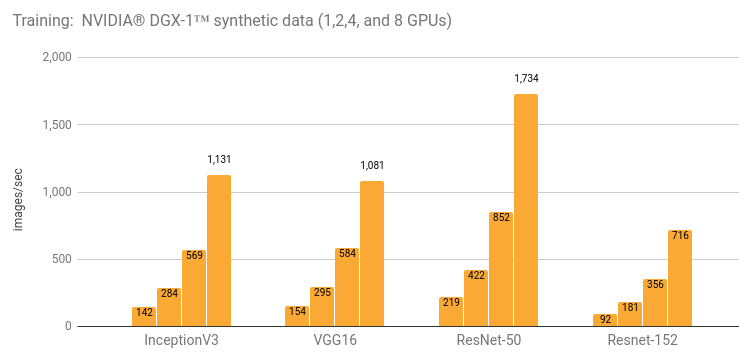
\includegraphics[scale=0.5]{perf_summary_p100_single_server.png}
\end{figure}
详细的额外的结果在\href{https://www.tensorflow.org/performance/benchmarks#details_for_nvidia_dgx-1tm_nvidia_tesla_p100}{Details for NVIDIA® DGX-1 (NVIDIA TeslaP100)}
\begin{figure}[H]
	\centering
	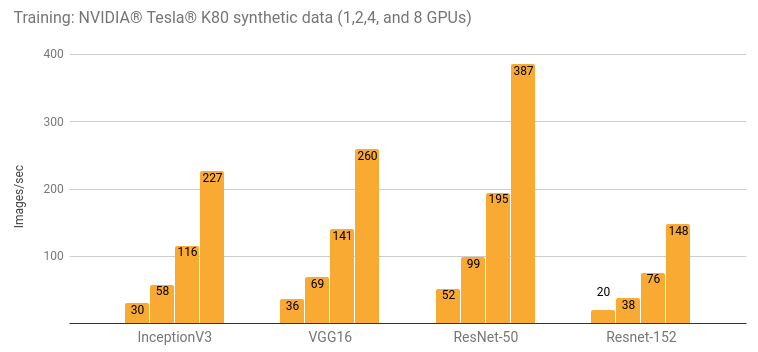
\includegraphics[scale=0.5]{perf_summary_k80_single_server.png}
\end{figure}
详细的额外的结果在\href{https://www.tensorflow.org/performance/benchmarks#details_for_google_compute_engine_nvidia_tesla_k80}{Details for Google Compute Engine (NVIDIA Tesla K80) }和\href{https://www.tensorflow.org/performance/benchmarks#details_for_amazon_ec2_nvidia_tesla_k80}{ Details for Amazon EC2 (NVIDIA Tesla K80) }
\subsection{用Tesla K80分布式的训练}
\begin{figure}[H]
	\centering
	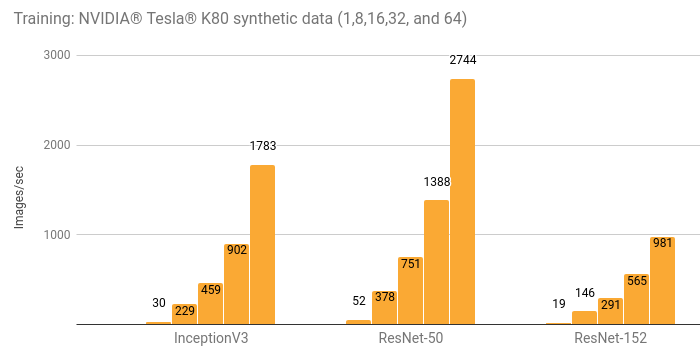
\includegraphics[scale=0.5]{perf_summary_k80_aws_distributed.png}
\end{figure}
详细的信息在\nameref{subsec:1}
\subsection{结合真是数据训练比较}
\begin{figure}[H]
	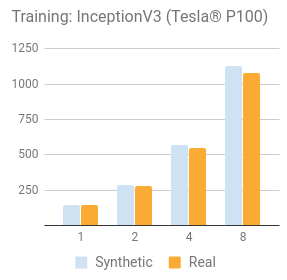
\includegraphics[scale=0.5]{perf_summary_p100_data_compare_inceptionv3}
	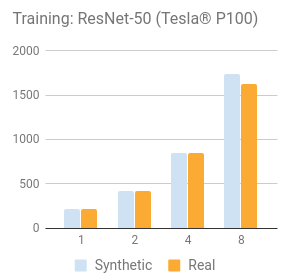
\includegraphics[scale=0.5]{perf_summary_p100_data_compare_resnet50}
\end{figure}
NVIDIA Tesla K80
\begin{figure}[H]
	\centering
	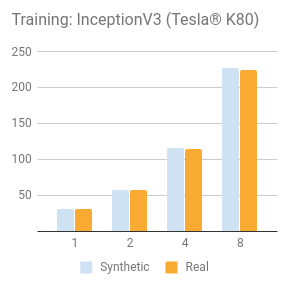
\includegraphics[scale=0.5]{perf_summary_k80_data_compare_inceptionv3.png}
	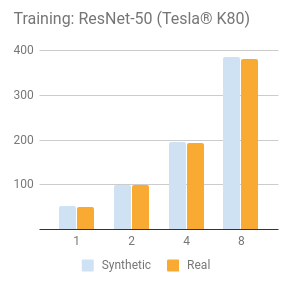
\includegraphics[scale=0.5]{perf_summary_k80_data_compare_resnet50.png}
\end{figure}
\subsection{详细的NVIDIA DGX-1(NVIDIA Tesla P100)}
\textbf{环境}\newline
\begin{itemize}
	\item 实例类型:NVIDIA DGX-1
	\item GPU:8x NVIDIA Tesla P100
	\item OS:通过Docker特使运行Ubuntu 16.0.4 LTS 
	\item CUDA/cuDNN"8.0/5.1
	\item TensorFlow GitHub b1e174e
	\item Benchmark GitHub hash:9165a70
	\item 构建命令:\lstinline[language=Bash]{bazel build -c opt --copt=-march="haswell" --config=cuda //tensorflow/tools/pip_package:build_pip_package}
	\item Disk:本地SSD
	\item Dataset:ImageNet
	\item Test Data:2017五月
\end{itemize}
用于模型的批大小和优化器在下表。另外在表中的批大小,Inception V3,ResNet-50,ResNet152和VGG16用于在批大小为32上测试,这些值在其他的结果章节:
\begin{table}[H]
	\begin{tabular}{|c|c|c|c|c|c|}
		选项&Inception v3&ResNet-50&ResNet-152&AlexNet&VGG16\\
		每个GPU批的大小&64&64&64&512&64\\
		优化器&sgd&sgd&sgd&sgd&sgd\\
	\end{tabular}
\end{table}
为每个模型配置:
\begin{table}[H]
	\begin{tabular}{|c|c|c|}
	模型&变量更新&本地变量设备\\
		InceptionV3 &参数服务器&cpu\\
		ResNet50 &参数服务器&cpu\\
		ResNet152 &参数服务器&cpu\\
		AlexNet &参数服务器&cpu\\
		VGG16 &参数服务器&cpu\\
	\end{tabular}
\end{table}
结果:
\begin{figure}[H]
	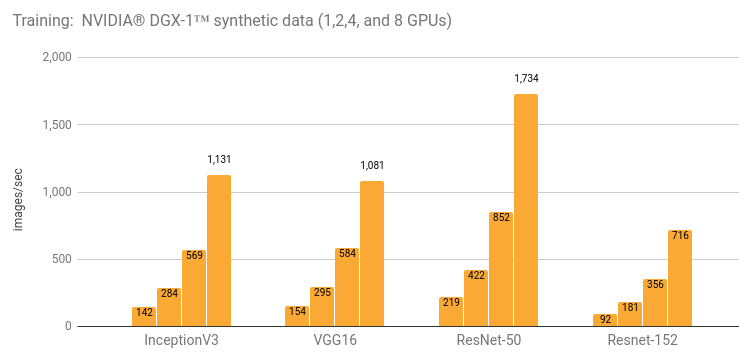
\includegraphics[scale=0.5]{perf_summary_p100_single_server.png}
	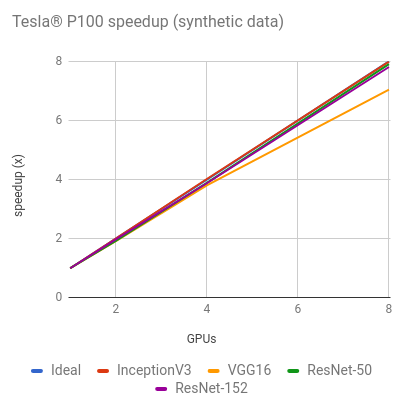
\includegraphics[scale=0.5]{perf_dgx1_synth_p100_single_server_scaling.png}
\end{figure}
训练聚合数据
\begin{table}H[]
	\begin{tabular}{|c|c|c|c|c|c|}
		GPUs	&InceptionV3	&ResNet-50	&ResNet-152	&AlexNet	&VGG16\\
		1	&142	&219	&91.8	&2987	&154\\
		2	&284	&422	&181	&5658	&295\\
		4	&569	&852	&356	&10509	&584\\
		8	&1131	&1734	&716	&17822	&1081\\
	\end{tabular}
\end{table}
训练真是数据
\begin{table}[H]
	\begin{tabular}{|c|c|c|c|c|c|}
		GPUs	&InceptionV3	&ResNet-50	&ResNet-152	&AlexNet	&VGG16\\
		1	&142	&218	&91.4	&2890	&154\\
		2	&278	&425	&179	&4448	&284\\
		4	&551	&853	&359	&7105	&534\\
		8	&1079	&1630	&708	&N/A	&898\\
	\end{tabular}
\end{table}
在8GPUs结合真实数据训练AlexNet从图上包含上面的表格最大化输入pipeline。
其他的结果

下面的结果每批32
\textbf{训练综合数据}
\begin{table}[H]
	\begin{tabular}{|c|c|c|c|c|}
		GPUs	&InceptionV3	&ResNet-50	&ResNet-152	&VGG16\\
		1	&128	&195	&82.7	&144\\
		2	&259	&368	&160	&281\\
		4	&520	&768	&317	&549\\
		8	&995	&1485	&632	&820\\
	\end{tabular}
\end{table}

训练真实数据
\begin{table}
	\begin{tabular}{|c|c|c|c|c|}
		GPUs	&InceptionV3	&ResNet-50	&ResNet-152	&VGG16\\
		1	&130	&193	&82.4	&144\\
		2	&257	&369	&159	&253\\
		4	&507	&760	&317	&457\\
		8	&966	&1410	&609	&690\\
	\end{tabular}
\end{table}
在Google Compute Engine上详情(NVIDIA Tesla K80)
\begin{itemize}
	\item  实例类型:n1-standard-32-k80x8
	\item  GPU:8 NVIDIA Tesla K80
	\item OS Ubuntu 16.04 LTS 
	\item CUDA/cuDNN:8.0/5.1
	\item TensorFlow GitHub hash:b1e174e
	\item Benchmark Github hash:9165a70
	\item 构建命令\lstinline[language=Bash]{bazel build -c opt --copt=-march="haswell" --config=cuda //tensorflow/tools/pip_package:build_pip_package}
	\item Disk:1.7TB共享SSD永久磁盘
	\item Dataset:ImageNet 
	\item Test Data:2017 5月
\end{itemize}
每个模型的批大小和优化器在下表中。另外批大小列在表格,InceptionV3和ResNet-50被测试一个batch为32,这些结果在其他章节。
\begin{table}[H]
	\begin{tabular}{|c|c|c|c|c|}
		Options	&InceptionV3	&ResNet-50	&ResNet-152	&AlexNet	&VGG16\\
		Batch size per GPU	&64	&64	&32	&512	&32\\
		Optimizer	&sgd	&sgd	&sgd	&sgd	&sgd\\
	\end{tabular}
\end{table}
这配置用于每个模型variable\_update等于parameter\_server和local\_parameter\_device等于cpu。
\textbf{结果}\\
\begin{figure}[H]
	\centering
	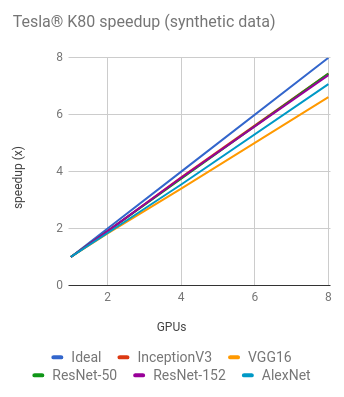
\includegraphics[scale=0.5]{perf_gce_synth_k80_single_server_scaling.png}
	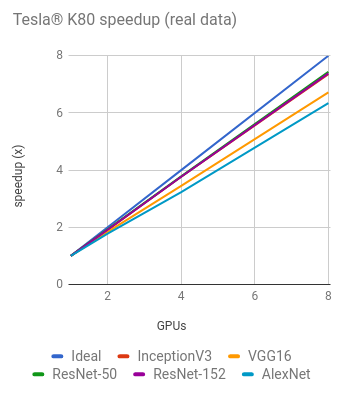
\includegraphics[scale=0.5]{perf_gce_real_k80_single_server_scaling.png}
\end{figure}
\begin{table}[H]
	\begin{tabular}{|c|c|c|c|c|}
		GPUs	&InceptionV3	&ResNet-50	&ResNet-152	&AlexNet	&VGG16\\
		1	&30.5	&51.9	&20.0	&656	&35.4\\
		2	&57.8	&99.0	&38.2	&1209	&64.8\\
		4	&116	&195	&75.8	&2328	&120\\
		8	&227	&387	&148	&4640	&234\\
	\end{tabular}
	\caption{Training synthetic data}
\end{table}
\begin{table}[H]
	\begin{tabular}{|c|c|c|c|c|c|}
		GPUs	&InceptionV3	&ResNet-50	&ResNet-152	&AlexNet	&VGG16\\
		1	&30.6	&51.2	&20.0	&639	&34.2\\
		2	&58.4	&98.8	&38.3	&1136	&62.9\\
		4	&115	&194	&75.4	&2067	&118\\
		8	&225	&381	&148	&4056	&230\\
	\end{tabular}
	\caption{训练真实数据}
\end{table}
\begin{table}[H]
	\begin{tabular}{|c|c|c|}
		GPUs	&InceptionV3 (batch size 32)	&ResNet-50 (batch size 32)\\
		1	&29.3	&49.5\\
		2	&55.0	&95.4\\
		4	&109	&183\\
		8	&216	&362\\
	\end{tabular}
	\caption{Training real data}
\end{table}
\subsection{Amazon Ec2详情(NVIDIA Tesla K80)}
环境
\begin{itemize}
	\item 实例类型:p2.8xlarge
	\item GPU:8x NVIDIA Tesla K80
	\item OS:Ubuntu16.0.4 LTS 
	\item CUDA/cuDNN:8.0/5.1
	\item TensorFlow Github hash:b1e174e
	\item Benchmark GitHub hash:9165a70
	\item 构建命令\lstinline[language=Bash]{bazel build -c opt --copt=-march="haswell" --config=cuda //tensorflow/tools/pip_package:build_pip_package}
	\item Disk:1TB Amazon EFS(brush 100MiB/sec for 12 hours,continous 50 MiB/sec)
	\item Dataset:ImageNet 
	\item TestData:2017 5月
\end{itemize}
用于每个模型的Batch size和优化器在下表。另外batch size列出在表格中,InceptionV3和ResNet-50用于在batch为32上测试。这些结果在其它章节
\begin{table}
\begin{tabular}{|c|c|c|c|c|}
	Options	InceptionV3	&ResNet-50	&ResNet-152	&AlexNet	&VGG16\\
	Batch size per GPU	&64	&64	&32	&512	&32\\
	Optimizer	&sgd	&sgd	&sgd	&sgd	&sgd\\
\end{tabular}
\end{table}
用于每个模型的配置
\begin{table}[H]
	\begin{tabular}{|c|c|c|}
		Model	&variable\_update	&local\_parameter\_device\\
		InceptionV3	&parameter\_server	&cpu\\
		ResNet-50	&replicated (without NCCL)	&gpu\\
		ResNet-152	&replicated (without NCCL)	&gpu\\
		AlexNet	&parameter\_server	&gpu\\
		VGG16	&parameter\_server	&GPUs \\
	\end{tabular}
\end{table}
 结果
 \begin{figure}[H]
	 \centering
	 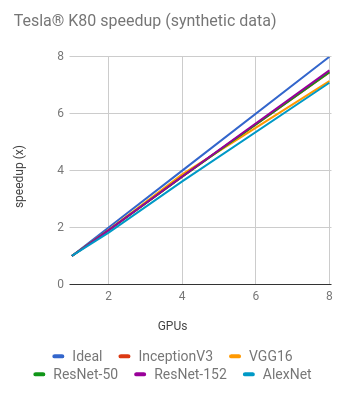
\includegraphics[scale=0.5]{perf_aws_synth_k80_single_server_scaling.png}
	 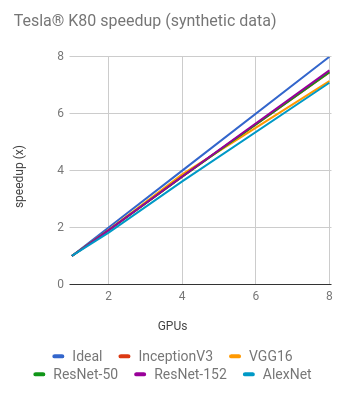
\includegraphics[scale=0.5]{perf_aws_synth_k80_single_server_scaling.png}
 \end{figure}
 \begin{table}[H]
	\begin{tabular}{|c|c|c|c|c|c|}
		GPUs	&InceptionV3	&ResNet-50	&ResNet-152	&AlexNet	&VGG16\\
		1	&30.8	&51.5	&19.7	&684	&36.3\\
		2	&58.7	&98.0	&37.6	&1244	&69.4\\
		4	&117	&195	&74.9	&2479	&141\\
		8	&230	&384	&149	&4853	&260\\
	\end{tabular}
	 \caption{Training synthetic data}
\end{table}
 \begin{table}[H]
	 \begin{tabular}{|c|c|c|c|c|c|}
		 GPUs	&InceptionV3	&ResNet-50	&ResNet-152	&AlexNet	&VGG16\\
		 1	&30.5	&51.3	&19.7	&674	&36.3\\
		 2	&59.0	&94.9	&38.2	&1227	&67.5\\
		 4	&118	&188	&75.2	&2201	&136\\
		 8	&228	&373	&149	&N/A	&242\\
	 \end{tabular}
 \end{table}
 结合8GPU从图上和表格训练真实数据因为我们的RFS设置没有提供足够的吞吐量。
 
 其他的结果
 \begin{table}[H]
	\begin{tabular}{|c|c|c|}
		GPUs	&InceptionV3 (batch size 32)	&ResNet-50 (batch size 32)\\
		1	&29.9	&49.0\\
		2	&57.5	&94.1\\
		4	&114	&184\\
		8	&216	&355\\
	\end{tabular}
	 \caption{Training synthetic data}
\end{table}
 \begin{table}[H]
	\begin{tabular}{|c|c|c|}
		GPUs	&InceptionV3 (batch size 32)	&ResNet-50 (batch size 32)\\
		1	&30.0	&49.1\\
		2	&57.5	&95.1\\
		4	&113	&185\\
		8	&212	&353\\
	\end{tabular}
	 \caption{Training real data}
\end{table}
 \subsection{在Amazon EC2上(NVIDIA Tesla K80)}
 \begin{itemize}
	 \item Instance type: p2.8xlarge
         \item GPU: 8x NVIDIA® Tesla® K80
	 \item  OS: Ubuntu 16.04 LTS
	\item 	 CUDA / cuDNN: 8.0 / 5.1
	\item 	 TensorFlow GitHub hash: b1e174e
	\item 	 Benchmark GitHub hash: 9165a70
	\item 	\lstinline[language=Bash]{} Build Command: bazel build -c opt --copt=-march="haswell" --config=cuda //tensorflow/tools/pip_package:build_pip_package}
	\item 	 Disk: 1.0 TB EFS (burst 100 MB/sec for 12 hours, continuous 50 MB/sec)
	\item 	 DataSet: ImageNet
	\item	 Test Date: May 2017
 \end{itemize}
 用于测试的批和优化器在下表。另外批大小在表格中,InceptionV3和ResNet-50用于在批大小为32上测试。这结果在其它章节。
 \begin{table}[H]
	 \begin{tabular}{|c|c|c|c|c|}
		 Options	&InceptionV3	&ResNet-50	&ResNet-152\\
		 Batch size per GPU	&64	&64	&32\\
		 Optimizer	&sgd	&sgd	&sgd\\

	 \end{tabular}
 \end{table}
 用于每个模型的配置

\begin{table}
	\begin{tabular}{|c|c|c|c|}
		Model	&variable\_update	&local\_parameter\_device	&cross\_replica\_sync\\
		InceptionV3	&distributed\_replicated	&n/a	&True\\
		ResNet-50	&distributed\_replicated	&n/a	&True\\
		ResNet-152	&distributed\_replicated	&n/a	&True\\
	\end{tabular}
\end{table}
为了简化服务器设置,EC2实例(p2.8xlarge)运行在worker服务器上也运行在参数服务器上。参数服务器数量和worker服务器用:
\begin{itemize}
		\item InceptionV3:8实例/参数服务器
		\item ResNet50:(批大小为32)8实例/4参数服务器
		\item ResNet-152:8shili /4参数服务器
\end{itemize}
 结果
 \begin{figure}[H]
	 \centering
	 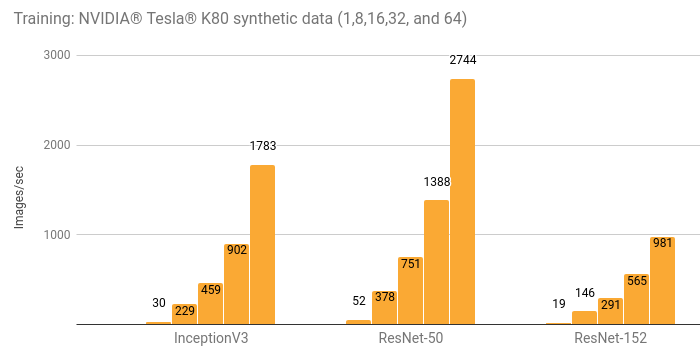
\includegraphics[scale=0.5]{perf_summary_k80_aws_distributed.png}
 \end{figure}
 \begin{figure}[H]
	 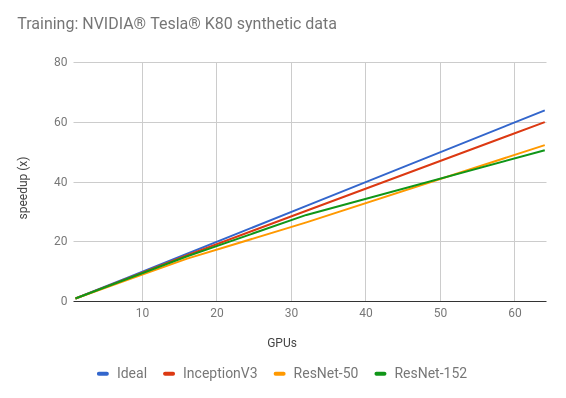
\includegraphics[scale=0.5]{perf_aws_synth_k80_distributed_scaling.png}
 \end{figure}
 \begin{table}
	 \begin{tabular}{|c|c|c|c|}
		 GPUs	&InceptionV3	&ResNet-50	&ResNet-152\\
		 1	&29.7	&52.4	&19.4\\
		 8	&229	&378	&146\\
		 16	&459	&751	&291\\
		 32	&902	&1388	&565\\
		 64	&1783	&2744	&981\\
	 \end{tabular}
 \end{table}
 其他结果
 \begin{figure}[H]
	 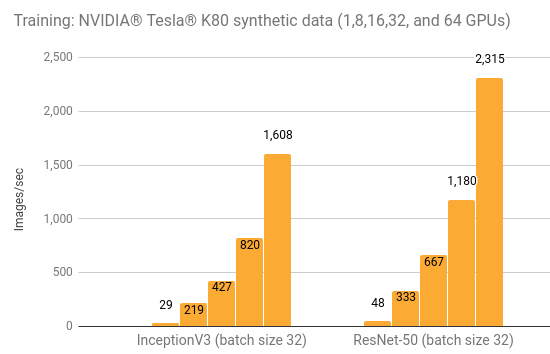
\includegraphics[scale=0.5]{perf_aws_synth_k80_multi_server_batch32.png}
 \end{figure}
 \begin{table}[H]
	 \begin{tabular}{|c|c|c|}
		 GPUs	&InceptionV3 (batch size 32)	&ResNet-50 (batch size 32)\\
		 1	&29.2	&48.4\\
		 8	&219	&333\\
		 16	&427	&667\\
		 32	&820	&1180\\
		 64	&1608	&2315\\
	 \end{tabular}
 \end{table}
 \subsection{方法论}
 这个\href{https://github.com/tensorflow/benchmarks/tree/master/scripts/tf_cnn_benchmarks}{脚本}运行在多个平台生成上面的结果。\href{https://www.tensorflow.org/performance/performance_models}{High-Performance Models}如何执行脚本的例子的详细技术在脚本中。

 为了创建结果可重复,没个测试运行5次然后时间被平均。GPU运行在默认给定的平台。对于NVIDIA Tesla K80这意味着让\href{https://devblogs.nvidia.com/parallelforall/increase-performance-gpu-boost-k80-autoboost/}{GPU Boose},10warmup步被做然后下一个100步被平均。

\section{对于ML初学者的MNIST}
这个导航针对于对机器学习和TensorFlow生疏的读者。如果你知道MNIST,softmax回归,你最好查看\href{https://www.tensorflow.org/get_started/mnist/pros}{faster paced turotial}。开始任何导航前确保你安装了\href{https://www.tensorflow.org/install/index}{TensorFlow}。
当一个人学习如何编程,他们通常做的第一件事就是打印Hello World。MNIST对于机器学习就像编程的Hello World。

MNIST是一个简单的计算机视觉数据集,由像下面的手写数据组成:
\begin{figure}[H]
\centering

\includegraphics{MNIST.png}
\caption{mnist数据}
\end{figure}
它包含每个图片的标签,高数我们是那个数字。例如,上面的标签分别是5,0,4,1。

在这个导航中,我们将训练一个模型查看图像预测数字。我们的目标不是训练一个真正精巧的模型获取顶尖的性能,尽管我们将在稍后给你代码。但是不是使用TensorFlow简单研究。例如,我们将开始一个非常简单的称为Softmax回归的模型。

实际上代码很短,所有有趣的东西仅仅发生在三行。然而,对于理解它背后的想法却很重要:TensorFlow如何工作和机器学习核心概念。因为这,我们将分厂自己的介绍代码。
\subsection{关于这个导航}
这个导航是一个一行行的解释\href{https://www.github.com/tensorflow/tensorflow/blob/r1.4/tensorflow/examples/tutorials/mnist/mnist_softmax.py}{mnist\_softmax.py}发生了什么。你可以通过两种不同的方法使用这个导航:
\begin{itemize}
\item 当你读每一行解释的时候复制粘贴一行行的每个代码段到Python环境
\item 在你读整个解释致歉运行整个mnist\_softmax.py Python文件,使用导航理解你不清楚的每行代码
在这个导航你将完成:
\item 了解MNIST数据集和softmax回归
\item 创建一个函数模型用于识别,易于图片上的每个像素
\item 通过"看"样本使用TensorFlow训练模型识别数字(运行我们的TensorFlow会话做到)
\item 结合我们的测试数据检查模型的精度
\end{itemize}
\subsection{MNIST数据}
MNIST数据在\href{http://yann.lecun.com/exdb/mnist/}{Yann LeCun's website}。如果你从文档上复制粘贴代码,用下面两行代码开头自动下载读取数据:
\begin{pythoncode}
from tensorflow.examples.tutorials.mnist import input_data
mnist = input_data.read_data_sets("MNIST_data/", one_hot=True)
\end{pythoncode}
MNIST数据分为3部分:55,000训练数据(mnist.train),10,000测试数据(mnist.test)和5,000验证数据(mnist.validation)。这分割很重要:它是机器学习中的基础用来分割数据以至于在没有学习的数据上学到实际上的范化。

正如 我们之前提到的,每个MNIST数据有两部分:手写数字的图片和对应的标签。我们将称为图像"x"和标签"y"。训练集和测试机都包含图像和对应的标签;例如训练图像是mnist.train.images训练标签是mnist.train.labels。

每张图片有$28\times28$像素,我们可以将他解释为一个数组:
\begin{figure}[H]
\centering
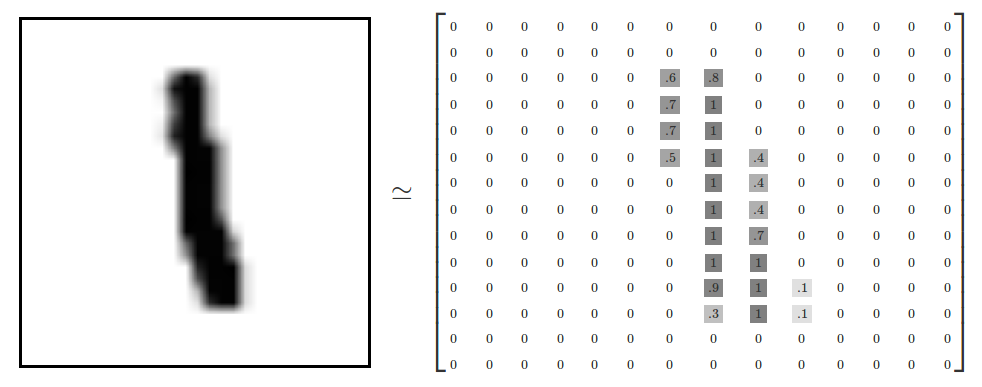
\includegraphics[scale=0.2]{MNIST-Matrix.png}
\caption{图片和对应的矩阵}
\end{figure}
我们可以展开这个数组为一个$28\times28=784$个数的向量。我们如何展开数组不重要只要它和图像一致即可。从这个观点,MNIST图像仅仅是一个\href{https://colah.github.io/posts/2014-10-Visualizing-MNIST/}{very rich structure }784维的向量空间。(警告:计算加强可视化)

展开市局丢掉了图像的2D结构,这很不好?使得最佳的计算机视觉方法利用这个结构,我们将在后面的导航中看到。但是简单的方法softmax回归将在这里使用。

结果时mnist.train.images是一个形状为[55000,784]的tensor(n维)。第一个为都市图像的索引,第二个是索引对应的图像像素。图像中的像素每个tensor的输入是一个0或者1。
\begin{figure}[H]
\centering

\includegraphics[scale=0.2]{mnist-train-xs.png}
\caption{图像维度}
\end{figure}
每个MNIST中的图像有一个对应的标签,一个0-9的数字,为了达到导航的目的,我们转化我们的标签为“one-hot vector”。一个one-hot向量是一个多数维度上为0,一个维度上1的向量。这种情况下,第n个数字表示维度中第n位置为1.例如3应该是[0,0,0,1,0,0,0,0,0,0]。结果mnist.train.labels是一个[55000,10]的浮点数组。
\begin{figure}[H]
\centering

\includegraphics[scale=0.2]{mnist-train-ys.png}
\caption{one-hot vector}
\end{figure}
现在我们准备开始我们的模型。
\subsection{Softmax回归}
我们知道在MNIST中的每张图片是0-9的手写体。因此给定一张图片仅仅只有10个可能。我们想能查看一张图片给定每张图片的概率。例如,我们的模型也许查看图像9 80\%确定是9,5\%确定为8其他的可能性很小因为模型不能100\%确定。

对这个经典的问题softmax恢复是一个自然,简单的模型。如果你想复制概率给一个对象成为多个不同对象中的一个,softmax做的就是这个,因为softmax给0-1的输出。在之后当我们训练更加精妙的模型,最后的步骤将是一个softmax操作。

一个softmax回归有两部:首先我们添加在确定类别中的输入,然后我们转化输出概率。为了总结一个类别的概率,如果它被支持我们权衡像素强度。

下面的图显示了从这些类别权衡一个模型。红色表示负权重,蓝色表示正权重。

\begin{figure}[H]
\centering
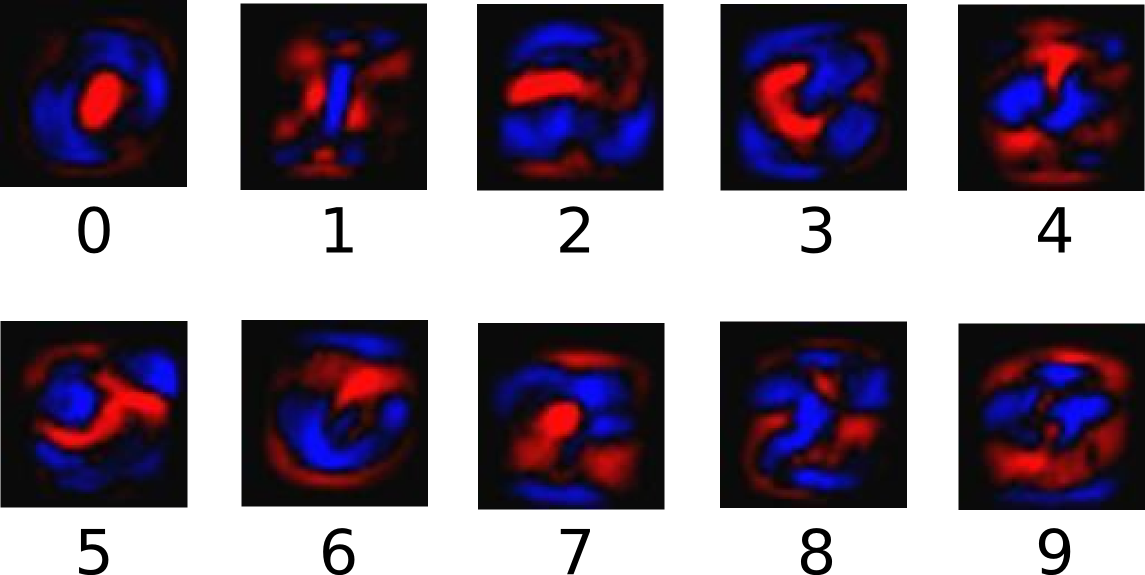
\includegraphics[scale=0.2]{softmax-weights.png}
\caption{softmax手写体}
\end{figure}
我们添加额外的偏执。基本上,我们想能说一些事更可能和输入独立。结果时给定输入x了类别i结果是:
\[evidence_i = \sum_{j}W_{i,j}x_j+b_i\]
这里的$W_i$是权重$b_i$是类别i偏置,j是在我们的输入图像x上的求和的索引。我们使用softmax转化evidence为我们的预测概率y:
\[y=softmax(evidence)\]
这里的softmax作为一个激活函数或者链接函数,输出我们线性函数为我们想要的。在这种情况下,概率分布在10个类别上。我们可以认为转化依据为我们输入每个类别的概率,定义如下:
\[softmax(evidence)=normalize(exp(evidence))\]
如果你展开方程,你得到:
\[softmax(evidence)_i = \frac{exp(evidence_i)}{\sum_jexp(evidence_j)}\]
但是首先考虑softmax方法京城很有用:指数输入和归一化。指数平均一个单元增加权重到任何假设。相反有更少的证据意味着假设获取之前前中的一部分。没哟偶假设有0或者负权重。fostmax然后归一化权重,以至于相加为1。形成一个可用的概率分布。(为了说明softmax函数,查看Michael Nielsen的数的\href{http://neuralnetworksanddeeplearning.com/chap3.html#softmax}{章节},完全的交互式可视化。)

你可以想下面画softmax回归,尽管有更多的x。对于每个输入,我们计算x的加权和加上偏执使用softmax。
\begin{figure}[H]
\centering
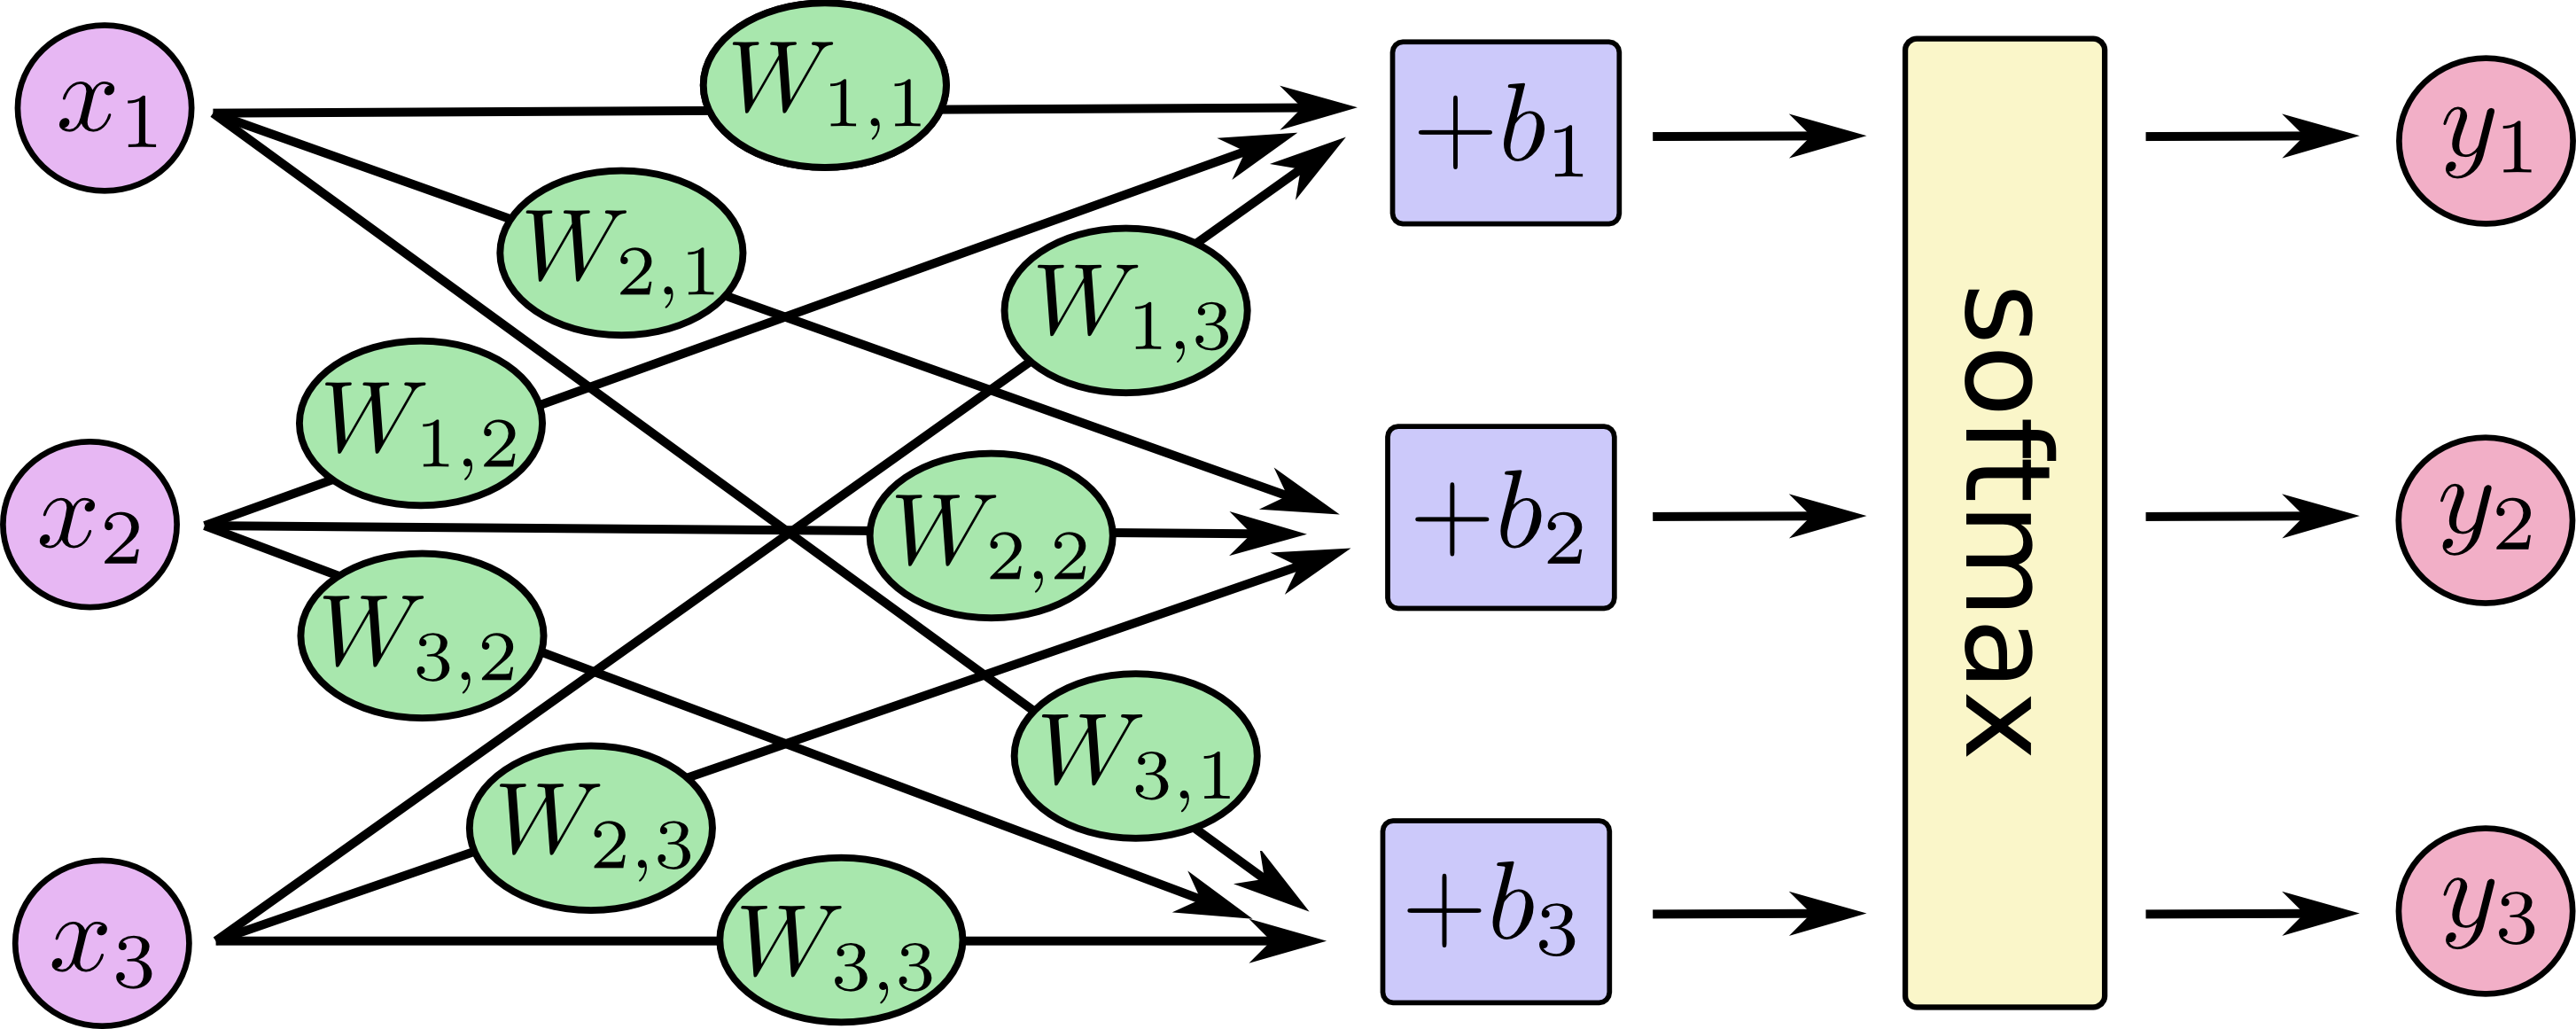
\includegraphics[scale=0.1]{softmax-regression-scalargraph.png}
\caption{softmax计算过程}
\end{figure}
如果你写为方程,你得到:
\begin{figure}[H]
\centering
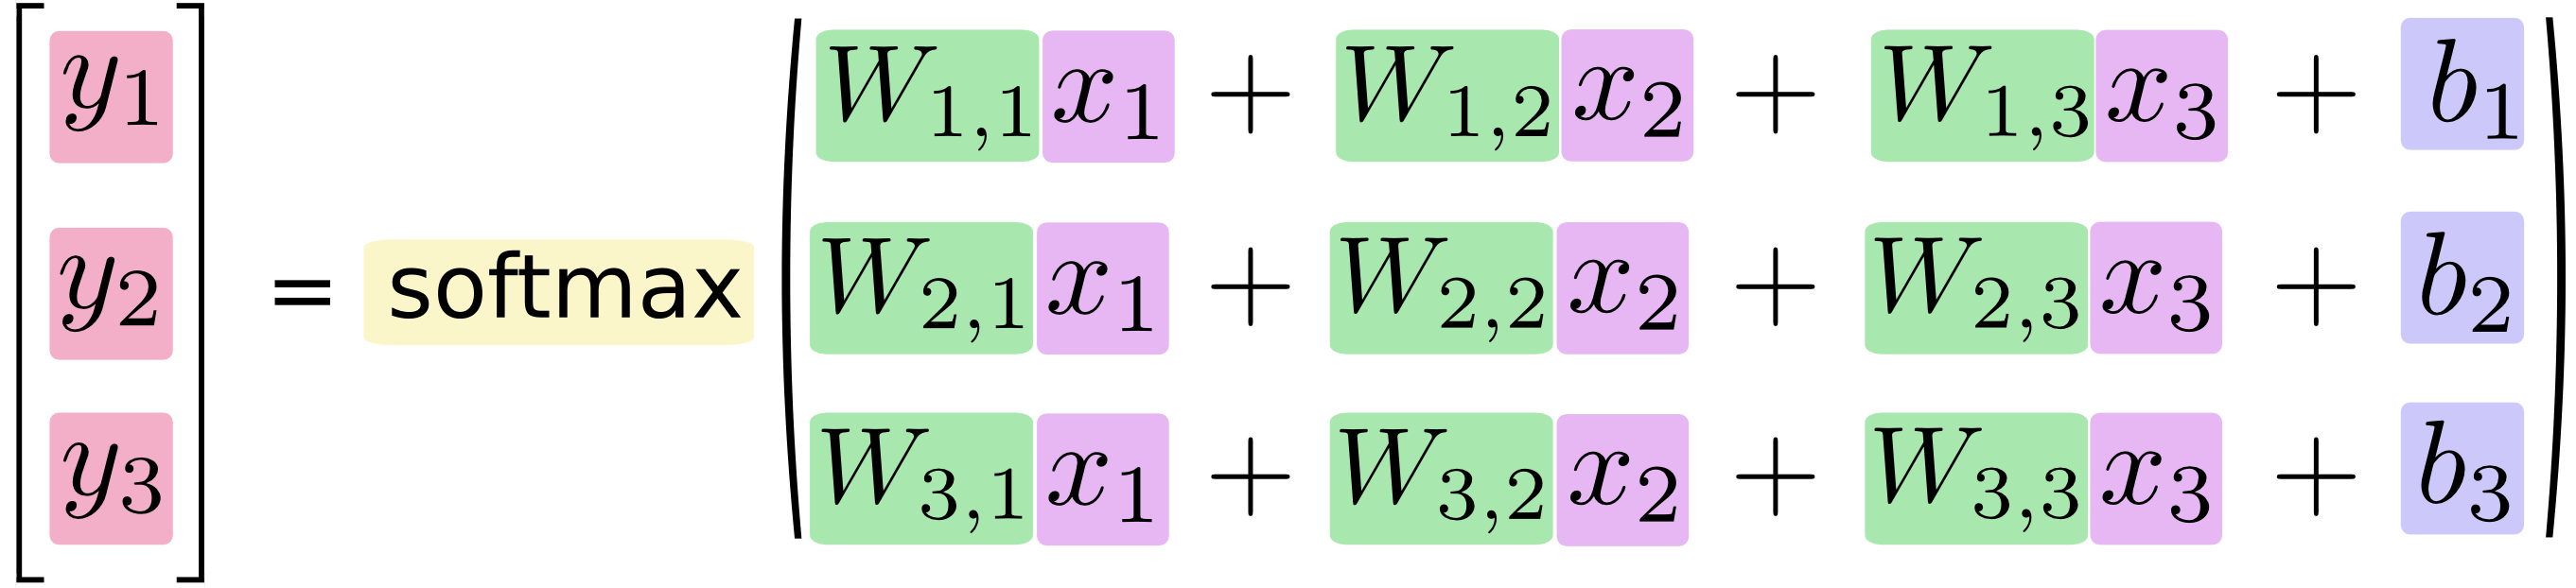
\includegraphics[scale=0.1]{softmax-regression-scalarequation.png}
\caption{softmax 方程}
\end{figure}
我们可以向量化这个过程,转变他为一个矩阵惩罚和向量加。这对于高效计算很有用(它总是一个有用的思考方法)。
\begin{figure}[H]
\centering
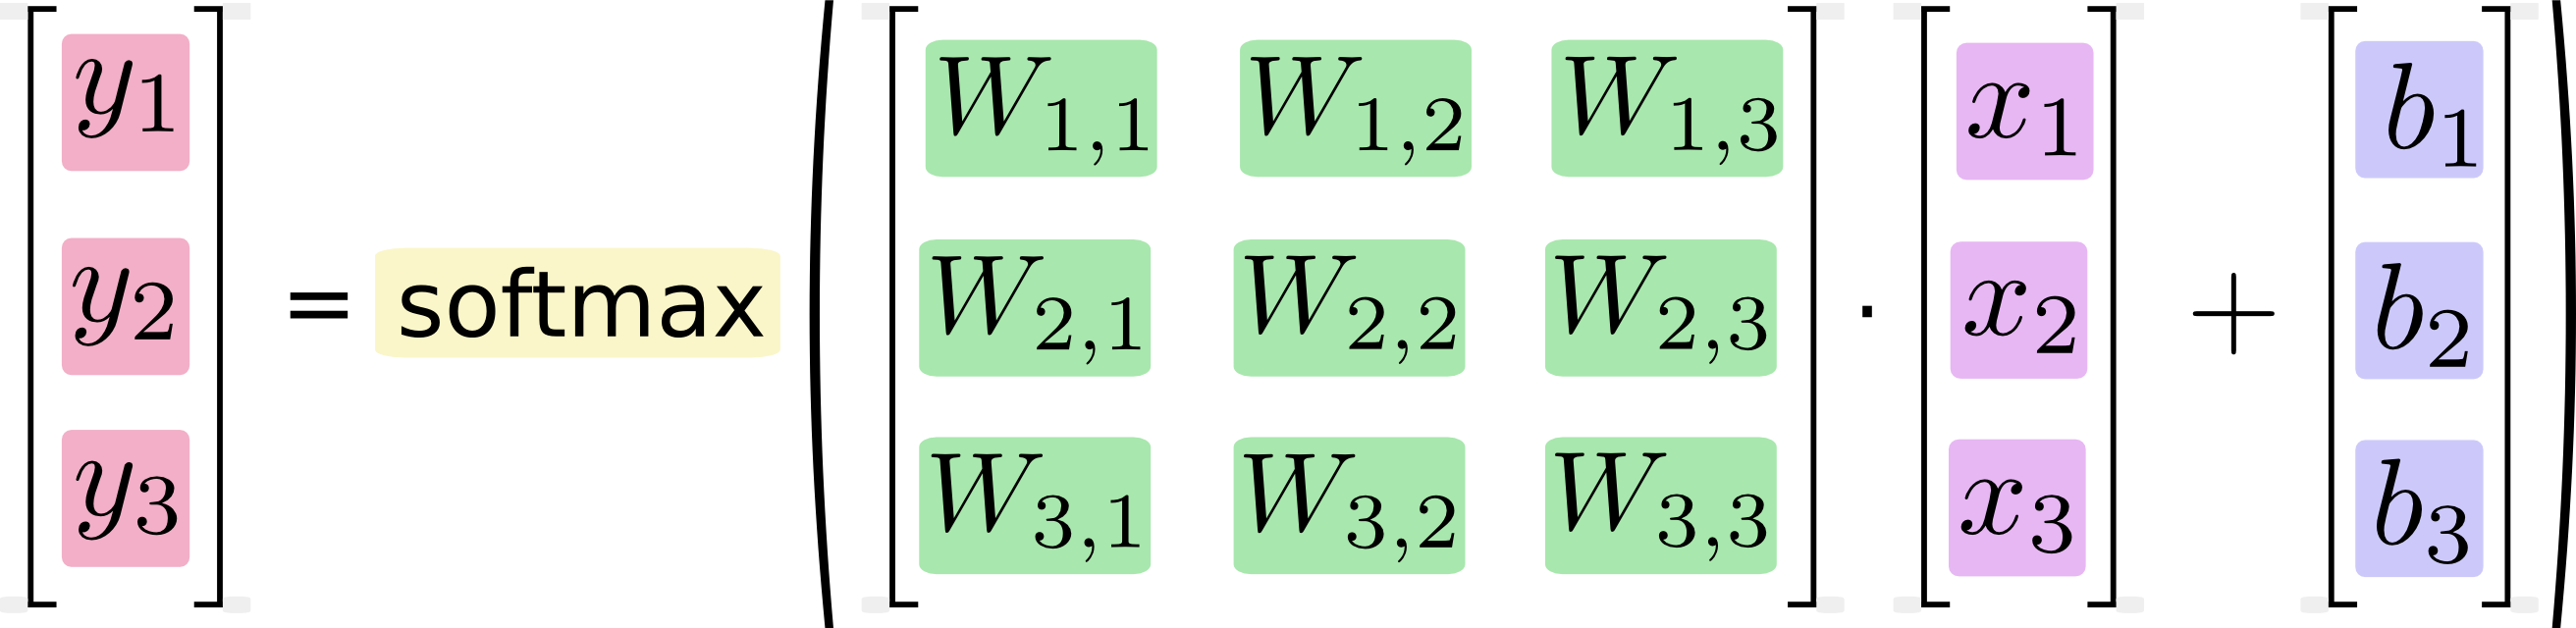
\includegraphics[scale=0.1]{softmax-regression-vectorequation.png}
\caption{向量化的softmax}
\end{figure}
更加简洁的你可以这样写:
\[y=fostmax(Wx+b)\]
现在我们使用TensorFlow转化它。
\subsection{实现回归}
为了在Python中进行的数值计算,我们通常使用一个\href{http://www.numpy.org/}{NumPy}库在Python外使用其他其他语言的高效实现做代价高昂的矩阵乘法操作。不幸的是转化每个操作会Python的时候依然有一些开销。如果你在GPU或者是分布式环境(这里我们转化数据代价很高)中使用是开销特别大。

TensorFlow也在Python外做了提升,但是对于减小开销减少有一点作用。想不语从Python运行的代价,TensorFlow让我们在Python外描述交互的操作。(这样的方法可以在一些机器学习库中看到)

为了使用TensorFlow,首先导入他。
\begin{ipythoncode}
import tensorflow as tf 
\end{ipythoncode}
我们通过符号变量描述交互的操作,让我们创建一个:
\begin{ipythoncode}
x = tf.placeholder(tf.float32, [None, 784])
\end{ipythoncode}
x没有指定值。是一个当我们要求TensorFlow运行时放置值的placholder。我们想能输入任意数量的MNIST图像,每张图像展开为784维(这里的None意味着这一维度可以为任意长度)
我们也需要权重和偏执用于计算。我们可以想象这些为额外的输入,但是TensorFlow有更好的处理方法:Variable。一个Variable是在TensorFlow图上的交互操作的一个可修改的tensor。他可以通过计算使用和修改。对于机器学习应用,一个常规的模型参数为Variable。
\begin{pythoncode}
W = tf.Variable(tf.zeros([784, 10]))
b = tf.Variable(tf.zeros([10]))
\end{pythoncode}
我们通过tf.Variable创建这些Variable初始化variable的值:在这种情况下,我们初始化W和b作为全0 tensor。因此我们将学习W和b。他们初始化为什么不重要。注意W形状为[784,10]因为我们想乘784维图像向量生成10维不同类别可信向量。b形状为[10]因此可以添加到输出。我们可以用一行定义实现我们的模型:
\begin{pythoncode}
y = tf.nn.softmax(tf.matmul(x, W) + b)
\end{pythoncode}
首先我们用tf.matmul(x,w)乘上x和W。它可我们方程用颠倒了这里是$Wx$作为结合多输入一个处理x为2D tensor的技巧。我们然后添加b最后使用tf.nn.softmax

这里我们使用了一行定义我们的模型,之后的一些行设置。这是不是因为TensorFlow设计就是为了做一个特别容易的regression:它仅仅是一个灵活的描述一些种类数值计算的方法,通过机器学习模型护理方针。一旦定义,我们的模型可以再不同的设备上运行:你的电脑的CPU,GPU甚至手机!

\subsubsection{训练}
为了定义我们的模型,我们需要定义什么方法对我们的模型来说很好。实际上机器学习中我们通常定义它意味着模型将变差。我们调用这个cost或者loss表达我们的模型和我们想要的输出之间的差距。我们尝试最小化误差,误差越小,模型越好。

通常,很简单的决定模型损失的函数为交叉熵(cross-entropy),交叉熵在信息论中提出考虑信息压缩编码,但是在一些淋雨,想机器学习领域变成了一个重要的想法,如下定义
\[H_y'(y)=-\sum_iy_i'log(y_i)\]
这里的y是我们的预测的概率分布,$y'$是真是的分布(数字的One-hot向量)。简单说交叉熵是衡量我们的预测对于真实的描述有多搞笑。详细的交叉熵介绍超过了这个导航范围,但是值得\href{https://colah.github.io/posts/2015-09-Visual-Information}{理解}。

为了实现交叉熵我们需要添加一个新的placeholder到输入正确的回答:
\begin{pythoncode}
y_ = tf.placeholder(tf.float32, [None, 10])
\end{pythoncode}
然后我们可以实现交叉熵函数$-\sum y'log(y)$:
\begin{pythoncode}
cross_entropy = tf.reduce_mean(-tf.reduce_sum(y_ * tf.log(y), reduction_indices=[1]))
\end{pythoncode}
首先,tf.log计算每个元素y的对数。下一步,我们乘上每个输入$y\_$和对应的tf.log(y)。然后tf.reduce\_sum添加元素在y的第二维,由于reduction\_indices=[1]参数。最后,tf.redce\_mean计算所有在batch中的样本的均值。

注意在源代码中,我们没有使用这个公式,因为这是数值不稳定的。取而代之的是我们shiyongtf.nn.softmax\_cross\_entropy\_with\_ligits在为最这话的logits(例如我们调用softmax\_cross\_entropy\_with\_logits在tf.matmul(x,W)+b)上,因为在更数值稳定函数内部计算softmax激活。在你的代码中,考虑使用tf.nn.softmax\_cross\_entropy\_with\_logits代替。
现在我们知道我们想让我们的模型做什么,对TensorFlow训练来说很容易。因为TensorFlow知道我们的整个计算图,这可以通过\href{https://colah.github.io/posts/2015-08-Backprop}{反向传播}搞笑的决定你的变量如何影响你想最小化的loss。这可以使用你的优化算法又该边疆减少loss。
\begin{pythoncode}
train_step = tf.train.GradientDescentOptimizer(0.5).minimize(cross_entropy)
\end{pythoncode}
在这种强狂下,我们要求TensorFlow通过学习率0.5的\href{https://en.wikipedia.org/wiki/Gradient_descent}{梯度下降算法}最小化交叉熵。梯度下降算法是一个简单的处理,这里TensorFlow简单的在cost见效的方向转变每个变量一点点。但是TensorFlow也提供\href{https://www.tensorflow.org/api_guides/python/train#Optimizers}{一些其他的优化算法}和上面一样简单的一行。

TensorFlow在这里做了什么,背后的机制是添加新的操作到图上实现反向传播和梯度下降。然后它给你返回一个操作,当运行的时候,体恤下降训练,轻微的转变你的变量减少损失。

我们可以在InteractiveSession启动模型:
\begin{pythoncode}
sess = tf.InteractiveSession()
\end{pythoncode}
我们首先必须创建一个操作初始化我们创建的变量:
\begin{pythoncode}
tf.global_variables_initializer().run()
\end{pythoncode}
让我们训练,我们将训练100次!
\begin{pythoncode}
for _ in range(1000):
  batch_xs, batch_ys = mnist.train.next_batch(100)
	  sess.run(train_step, feed_dict={x: batch_xs, y_: batch_ys})
\end{pythoncode}
循环的每一步,我们从我们的训练集上得到100个batch随机的数据点。我们运行train\_step输入批数据代替placeholder。

使用晓得batch随机数据成为随机训练,在这种情况下。最佳的我们想在每部使用所有的我们的数据因为浙江给我们一个更好的关于我们应该做什么的理解。但是这代价带。因此,作为替代,我们每次用一个不同的子集。作者有相同的好处代价更低。
\subsubsection{评估我们的模型}
我们的模型效果怎样?
首先让我们找出预测争取的标签。tfargmax是一个极其有用的函数给你沿着一个轴最高的输入tensor的索引。例如,tf.argmax(y,1)是我们的模型对于输入的认为最可能的标签,然而tf.ragmax(y\_1,1)是正确的标签。我们可以使用tf.equal检查是否我们的预测和真实情况匹配。
\begin{pythoncode}
correct_prediction = tf.equal(tf.argmax(y,1), tf.argmax(y_,1))
\end{pythoncode}
这给我们一个boolean列表。为了决定什么部分是正确的,我们转化为浮点数然后平均。例如[True,False,True,True]将被转化为[1,0,1,1]为0.75。
\begin{pythoncode}
accuracy = tf.reduce_mean(tf.cast(correct_prediction, tf.float32))
\end{pythoncode}
最后我们获取我们的测试集上的精度:大约92\%
\begin{pythoncode}
print(sess.run(accuracy, feed_dict={x: mnist.test.images, y_: mnist.test.labels}))
\end{pythoncode}
这很好?不,事实上,很差。这是因为我们使用了一个非常简单的模型。结合一些改变,我们可以得到97\%。最好的模型可以达到99.7\%的精度(更多信息查看\href{https://rodrigob.github.io/are_we_there_yet/build/classification_datasets_results}{结果列表})

我们从这个模型学到的重要的。一球,如果你正对结果感到沮丧。查看\href{https://www.tensorflow.org/get_started/mnist/pros}{下一个导航}这里我们使用TensorFlow做了一些更好的,学习构建更多精妙的模型。

\end{document}
